\section{Experimental Results}
\subsection{Part 1: Hopper}
Figure~\ref{fig:part1-train-comparison} compares REINFORCE without baseline, REINFORCE with a constant baseline of 20, and the actor-critic variant over seeds 0, 42, and 99. All methods improve from the initial policy, but the curves remain noisy, as expected for policy-gradient training on Hopper. The constant baseline gives the strongest final training curve and reduces some early variance relative to plain REINFORCE. The actor-critic variant learns more slowly and reaches lower average returns in this implementation.

\begin{figure}[H]
\centering
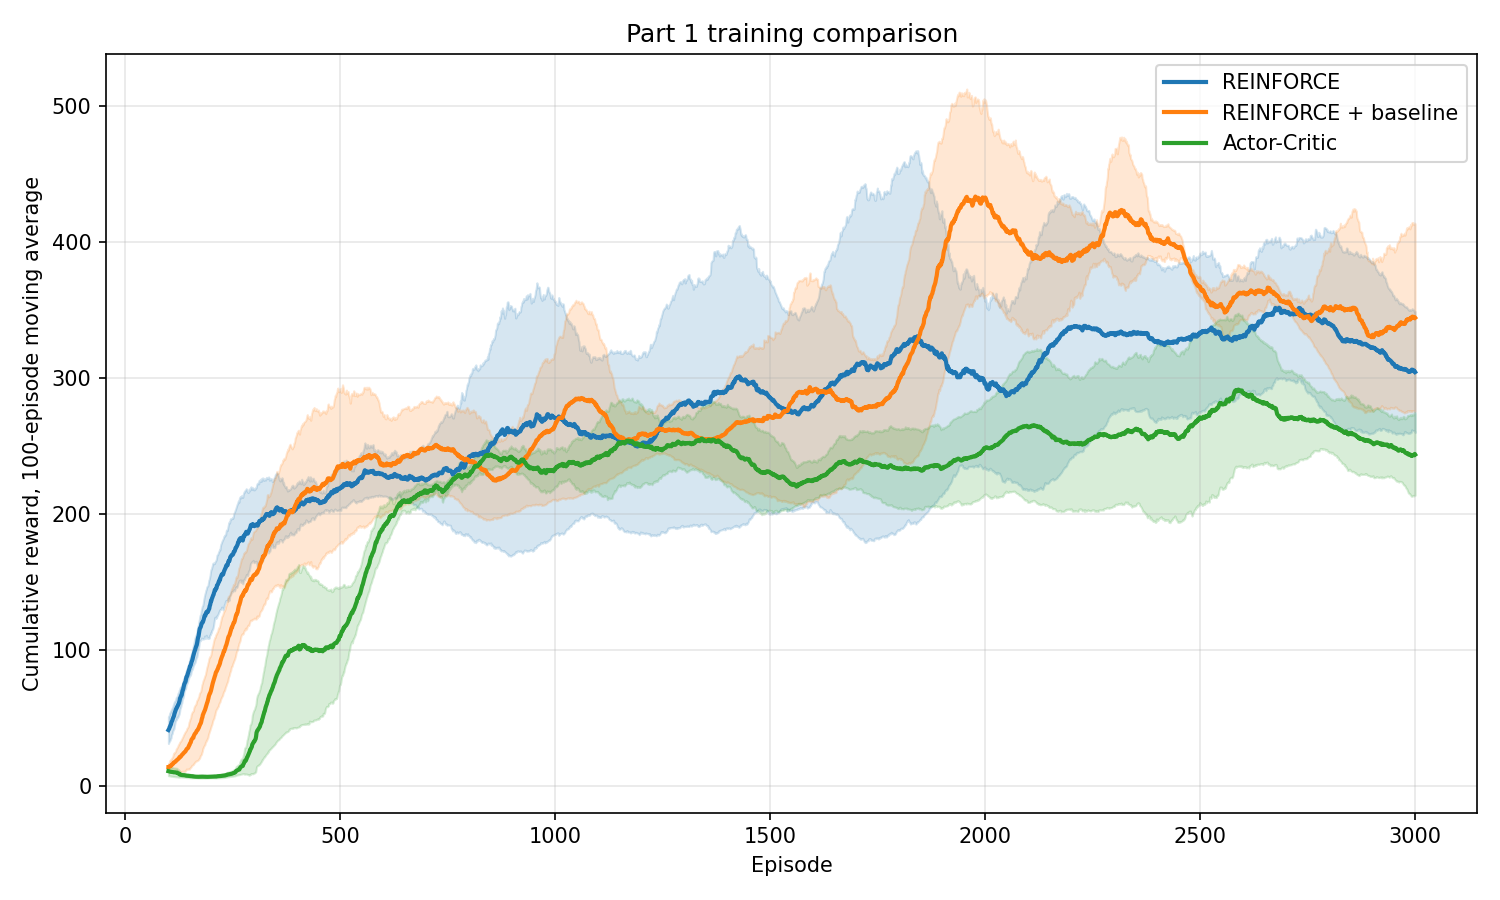
\includegraphics[width=\linewidth]{../part1/plots/comparison_train_mean_std.png}
\caption{Part 1 training comparison on \texttt{Hopper-v4}. Curves show the 100-episode moving average of cumulative reward, averaged over seeds 0, 42, and 99; shaded regions show variability across seeds.}
\label{fig:part1-train-comparison}
\end{figure}

\subsection{Part 2: PandaPush-v3}
For the second part of the project both PPO and SAC models were trained, however since the training of PPO was more unstable and it does not 
converge, only SAC was kept for further implemantations and evaluations.

\begin{figure}[H]
\centering
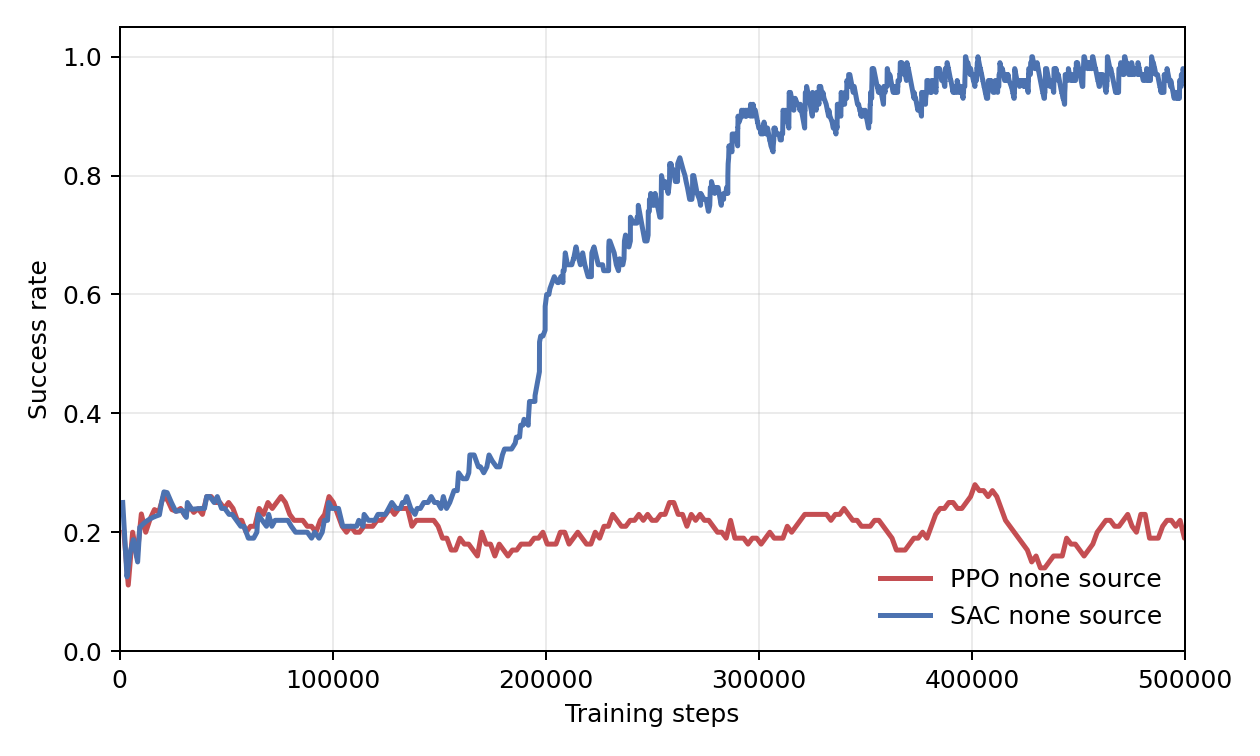
\includegraphics[width=\linewidth]{../part2/plots/ppo_sac_success_rate.png}
\caption{Training success-rate comparison on the source-domain \texttt{PandaPush-v3} task without domain randomization. The PPO curve corresponds to \texttt{PPO\_none\_source\_500k\_lr2e-4\_g095\_1}, while the SAC curve corresponds to \texttt{SAC\_none\_source\_500k\_2}.}
\label{fig:ppo-sac-success-rate}
\end{figure}

\subsection{Nominal Sim-to-Sim Evaluation}
The first section of table~\ref{tab:nominal-eval} reports aggregated 150-episodes evaluations (50 episodes per seed) generated from the saved SAC checkpoints. 
At the nominal target mass of 5 kg, the source-trained SAC policy already transfers well: 
the gap between source to source and source  to target is small when analyzing success rate.

\begin{table*}[t]
\centering
\small
\begin{tabular}{llccc}
\toprule
Model & Evaluation & Mean return & Std return & Success \\
\midrule
SAC source  & target (easy) & -1.740 & 7.917 & 97.3\%\\
SAC target  & target (easy) & -0.608 & 2.237 & 99.3\% \\
\midrule
SAC source \textbf{(Lower Bound)} & target (hard) & -12.762 & 19.722 & 72.0\% \\
SAC UDR hard target & target (hard) & -6.970 & 16.423 & 85.3\% \\
SAC UDR + friction source & target (hard) & -4.814 & 14.555 & 90.7\% \\
SAC ADR + friction source & target (hard) & -4.638 & 27.440 & 94.0\% \\
\bottomrule
\end{tabular}
\caption{Deterministic SAC evaluations aggregated over 150 episodes, using 50 episodes for each seed in $\{0,42,99\}$. The hard target samples mass from $\mathcal{U}(5,10)$ kg, object/table lateral friction from $\mathcal{U}(0.2,1.5)$, and object spinning friction from $\mathcal{U}(0,0.01)$.}
\label{tab:nominal-eval}
\end{table*}

\subsection{Harder Mass and Friction Evaluation}
Because nominal mass transfer was already strong, the evaluation was made harder by randomizing parameters at test time.
Table~\ref{tab:nominal-eval} uses mass sampled uniformly in $[5,10]$ kg, object/table lateral friction sampled in $[0.2,1.5]$, and object spinning friction sampled in $[0,0.01]$.
Under this harder protocol, the non-randomized source policy drops from 97.3\% to 72\% success on target. 
This result was used as Lower Bound for further experiments using domain randomization. 

A stronger target-distribution baseline was then obtained by training UDR directly on the target-domain intervals, with mass sampled from $\mathcal{U}(5,10)$~kg and lateral friction from $\mathcal{U}(0.2,1.5)$, matching the hard evaluation distribution exactly.
This model reaches 85.3\% success on the hard target over the same aggregated 150 episodes, improving over the non-randomized lower bound but remaining below the source-domain UDR and ADR policies.

\subsection{Domain Randomization: UDR and ADR}
In order to close the reality gap under hard evaluation, UDR and ADR policies were trained and tested.
The UDR policy trained with mass and friction randomization reaches 90.7\%.
Moreover, the ADR policy generalizes even better on unseen distribution, achieving 94\% of SR on the hard evaluation setting.
Although direct UDR training on the target-domain distribution is an intuitive strong baseline, both source-domain UDR and ADR outperform it under the current training budget.
Despite seeing the same distribution during training and evaluation, the UDR hard target model still performs worse than the ADR curriculum model.
The per-bin breakdown in Table~\ref{tab:udr-friction-bins} uses the same 150 hard-target evaluation episodes as Table~\ref{tab:nominal-eval}; ADR is stronger in every object-lateral-friction bin, and the largest gap appears at high table friction.

\begin{table}[H]
\centering
\small
\begin{tabular}{lccc}
\toprule
$\mu$ bin & $N$ & UDR hard SR & ADR SR \\
\midrule
\multicolumn{4}{l}{Object lateral friction} \\
$[0.20,\,0.46)$ & 33 & 90.9\% & 93.9\% \\
$[0.46,\,0.72)$ & 19 & 84.2\% & 89.5\% \\
$[0.72,\,0.98)$ & 33 & 78.8\% & 87.9\% \\
$[0.98,\,1.24)$ & 41 & 82.9\% & 100.0\% \\
$[1.24,\,1.50]$ & 24 & 91.7\% & 95.8\% \\
\midrule
\multicolumn{4}{l}{Table lateral friction} \\
$[0.20,\,0.46)$ & 25 & 92.0\% & 96.0\% \\
$[0.46,\,0.72)$ & 33 & 90.9\% & 97.0\% \\
$[0.72,\,0.98)$ & 38 & 86.8\% & 94.7\% \\
$[0.98,\,1.24)$ & 20 & 90.0\% & 90.0\% \\
$[1.24,\,1.50]$ & 34 & 70.6\% & 91.2\% \\
\midrule
Overall & 150 & 85.3\% & 94.0\% \\
\bottomrule
\end{tabular}
\caption{Friction-bin success rates for \texttt{models/SAC\_udr\_hard\_target\_500k/model.zip} and \texttt{models/SAC\_adr\_source\_500k/model.zip} on the hard target deterministic evaluation, aggregated over 150 episodes using 50 episodes for each seed in $\{0,42,99\}$. The hard target uses the same mass and friction randomization protocol as Table~\ref{tab:nominal-eval}.}
\label{tab:udr-friction-bins}
\end{table}
